\documentclass[11pt,a4paper]{article}

% ── FONTS ────────────────────────────────────────────────────
\usepackage{fontspec}
\setmainfont{Calibri}
\setsansfont{Calibri}
\newfontfamily{\hindifont}{Nirmala UI}[Script=Devanagari]
\newcommand{\hindi}[1]{{\hindifont #1}}

% ── LAYOUT ───────────────────────────────────────────────────
\usepackage[top=2cm,bottom=2.5cm,left=2.2cm,right=2.2cm]{geometry}
\usepackage{graphicx}
\usepackage{xcolor}
\usepackage{tikz}
\usetikzlibrary{calc,shapes.geometric,arrows.meta,positioning,fit,backgrounds}
\usepackage{tcolorbox}
\tcbuselibrary{skins,breakable}
\usepackage{colortbl}
\usepackage{booktabs}
\usepackage{tabularx}
\usepackage{enumitem}
\usepackage{setspace}
\usepackage{fancyhdr}
\usepackage{titlesec}
\usepackage{hanging}
\usepackage{multicol}
\usepackage{hyperref}
\usepackage{microtype}
\usepackage{array}
\usepackage{caption}

\hypersetup{colorlinks=false,hidelinks}

% ── BRAND COLORS ─────────────────────────────────────────────
\definecolor{navyblue}{HTML}{003566}
\definecolor{gold}{HTML}{C9A84C}
\definecolor{lightgray}{HTML}{F4F6FB}
\definecolor{midgray}{HTML}{D0D6E2}
\definecolor{darkgray}{HTML}{4A4A4A}
\definecolor{accentteal}{HTML}{0077B6}
\definecolor{sectionbg}{HTML}{EEF2FA}
\definecolor{softgreen}{HTML}{E8F5E9}
\definecolor{darkgreen}{HTML}{2E7D32}

% ── SECTION HEADING ──────────────────────────────────────────
\newcommand{\navysectionbox}[1]{%
  \hspace{-2.2cm}%
  \colorbox{navyblue}{%
    \hspace{2.2cm}%
    \parbox[c][0.65cm]{\dimexpr\textwidth+2.0cm}{%
      {\fontsize{12}{14}\selectfont\color{white}\strut\textbf{#1}}%
    }%
  }%
}

\titleformat{\section}[block]{\normalfont}{}{0em}{\navysectionbox}
\titlespacing*{\section}{-2.2cm}{16pt}{8pt}

\titleformat{\subsection}[block]
  {\normalfont\bfseries\fontsize{10.5}{13}\selectfont\color{navyblue}}
  {}{0em}{}
\titlespacing*{\subsection}{0pt}{10pt}{2pt}

% ── HEADER / FOOTER ──────────────────────────────────────────
\setlength{\headheight}{20pt}
\pagestyle{fancy}
\fancyhf{}
\fancyhead[L]{\footnotesize\color{navyblue}\textbf{AIGGPA Bhopal}
  \quad\textbar\quad IT Utilisation Assessment}
\fancyhead[R]{\footnotesize\color{navyblue}April 2026}
\fancyfoot[C]{\footnotesize\color{navyblue}\thepage}
\renewcommand{\headrulewidth}{0.4pt}
\renewcommand{\headrule}{\color{navyblue}\hrule width\headwidth height\headrulewidth}
\renewcommand{\footrulewidth}{1.5pt}
\renewcommand{\footrule}{\color{gold}\hrule width\headwidth height 1.5pt}

% ── CUSTOM BOXES ─────────────────────────────────────────────
\newtcolorbox{goldbox}{
  colback=gold!10, colframe=gold, boxrule=0.7pt, arc=3mm,
  left=10pt,right=10pt,top=8pt,bottom=8pt,breakable}

\newtcolorbox{navybox}{
  colback=sectionbg,colframe=navyblue,boxrule=0.6pt,arc=3mm,
  left=10pt,right=10pt,top=8pt,bottom=8pt,breakable}

\newtcolorbox{greenbox}{
  colback=softgreen,colframe=darkgreen,boxrule=0.6pt,arc=3mm,
  left=10pt,right=10pt,top=8pt,bottom=8pt,breakable}

\newtcolorbox{streamboxa}{
  colback=lightgray,colframe=accentteal,boxrule=1.2pt,arc=3mm,
  lefttitle=8pt,toptitle=4pt,bottomtitle=4pt,
  left=8pt,right=8pt,top=6pt,bottom=6pt,
  title={\bfseries\fontsize{9}{11}\selectfont\color{white}
    Stream A \textbullet{} Department Officials},
  colbacktitle=accentteal,breakable}

\newtcolorbox{streamboxb}{
  colback=lightgray,colframe=navyblue,boxrule=1.2pt,arc=3mm,
  lefttitle=8pt,toptitle=4pt,bottomtitle=4pt,
  left=8pt,right=8pt,top=6pt,bottom=6pt,
  title={\bfseries\fontsize{9}{11}\selectfont\color{white}
    Stream B \textbullet{} IT Department},
  colbacktitle=navyblue,breakable}

% ── LISTS ────────────────────────────────────────────────────
\setlist[itemize]{leftmargin=1.2em,itemsep=2pt,topsep=3pt}
\setlist[enumerate]{leftmargin=1.4em,itemsep=2pt,topsep=3pt}

% ─────────────────────────────────────────────────────────────
\begin{document}
\onehalfspacing

% ═════════════════════════════════════════════════════════════
%  COVER PAGE
% ═════════════════════════════════════════════════════════════
\thispagestyle{empty}
\begin{tikzpicture}[remember picture,overlay]
  \fill[navyblue] (current page.south west) rectangle (current page.north east);
  \fill[gold] (current page.south west)
    rectangle ($(current page.south east)+(0,1.1cm)$);
  \fill[white] ($(current page.south west)+(0,1.1cm)$)
    rectangle ($(current page.south east)+(0,11.8cm)$);
  \fill[accentteal!80]
    ($(current page.south west)+(0,11.8cm)$) --
    ($(current page.south east)+(0,11.8cm)$) --
    ($(current page.south east)+(0,13.2cm)$) --
    ($(current page.south west)+(0,12.4cm)$) -- cycle;
\end{tikzpicture}

\vspace*{6cm}
\begin{center}
  \fontsize{8.5}{10}\selectfont\color{gold!80}
  \textbf{\MakeUppercase{Institutional Research Proposal}}\\[0.7em]
  \fontsize{26}{31}\selectfont\bfseries\color{white}
  Assessment of IT Tool\\[0.15em]
  Utilisation Among\\[0.15em]
  Government Officials\\[0.9em]
  \fontsize{11}{14}\selectfont\color{midgray}
  \hindi{सरकारी अधिकारियों द्वारा आईटी उपकरणों के उपयोग का आकलन}
\end{center}

\vspace*{2.5cm}

\begin{tikzpicture}[remember picture,overlay]
  \node[anchor=south west] at ($(current page.south west)+(2.2cm,1.5cm)$){%
    \begin{minipage}{14cm}
      \footnotesize\color{darkgray}
      \begin{tabular}{@{}ll@{}}
        \textbf{Investigator:} & Aryan Kori \\[3pt]
        \textbf{Institution:}  & AIGGPA, Bhopal \\[3pt]
        \textbf{Departments:}  & School Education \textbullet{} Health
                                 \textbullet{} Forest, Govt.\ of MP \\[3pt]
        \textbf{Date:}         & April 2026 \\
      \end{tabular}
    \end{minipage}%
  };
\end{tikzpicture}

\newpage

% ═════════════════════════════════════════════════════════════
%  BACKGROUND
% ═════════════════════════════════════════════════════════════
\section{Background}

\vspace{0.2cm}
Over the last few years, the Government of Madhya Pradesh has invested heavily in digital 
infrastructure through agencies like MAP-IT and NIC. This has led to a major rollout 
of digital platforms across the state’s key departments:

\begin{itemize}[leftmargin=1.4em]
  \item \textbf{School Education:} The Education Portal 3.0 is a massive system set up to 
    handle roughly 3.5 lakh teachers. It's supposed to cover everything 
    from transfers to simple daily attendance.\footnote{Government
    of Madhya Pradesh, School Education Department (2025). \url{https://sederp.educationportal3.in}.}
    But while the system is there, how much it's actually used in a block-level office is 
    often a different story.

  \item \textbf{Health:} Between HRMIS for staff management and NHM CHETNA for 
    training, there's a lot of tech in play. Recently, they even launched an AI chatbot, 
    ``Ayushman Sakhi,'' to help citizens find hospitals.

  \item \textbf{Forest:} This department is using satellite data for tracking 
    encroachments and has moved wildlife permitting to the MPOnline portal.
\end{itemize}

Even with all these platforms, what we see in local offices is that workflows 
still often run on paper registers and informal WhatsApp groups. It's not that 
the tech is bad, but there's a clear gap between what a system is built to do 
and the actual reality of how an official works on the ground (Heeks, 2003). 
AIGGPA's own training sessions often bring up the same point: officials know these 
tools exist, but they still find it easier to stick to their old ways. We need to 
actually map out where the bottlenecks are.

% ═════════════════════════════════════════════════════════════
%  RATIONALE
% ═════════════════════════════════════════════════════════════
\section{Rationale}

\vspace{0.2cm}

Getting officials to use these tools properly isn't just about modernizing—it's 
about making the state bureaucracy actually work faster. Right now, a huge 
chunk of IT budgets goes just into keeping legacy systems "alive" rather than 
making things more efficient (GAO, 2019). If we can bridge this gap, we can 
cut down the time officials spend on manual document processing that hasn't 
really changed in decades.

Instead of keeping records in scattered registers, moving to these digital 
portals lets the state make better, data-driven decisions. This study is about 
finding exactly where the flow breaks down so we can get the real value out 
of Madhya Pradesh's IT investments.

% ═════════════════════════════════════════════════════════════
%  CAPACITY BUILDING
% ═════════════════════════════════════════════════════════════
\section{Capacity Building Framework}

\vspace{0.2cm}

Mission Karmayogi has changed how training works in the government. It has moved us 
away from just learning basic rules to actual "role-based" skills. The DoPT 
now emphasizes the iGOT platform for this. Since AIGGPA is the main 
training institute for the state, this research will help us design better, 
more practical IT training modules. The goal is to make sure what we teach 
at AIGGPA actually helps an official when they go back to their desk.

% ═════════════════════════════════════════════════════════════
%  THEORETICAL FRAMEWORK
% ═════════════════════════════════════════════════════════════
\section{Theoretical Framework}

\vspace{0.2cm}

To understand why some officials avoid these tools while others use them, this 
study uses the \textbf{Unified Theory of Acceptance and Use of Technology (UTAUT)}. 
It's a solid framework for government work because it looks at both individual 
feelings and the workplace environment. We'll be looking at four main areas:

\begin{itemize}
  \item \textbf{Performance Expectancy (PE):} Does the official think the tool 
    actually makes their job easier?
  \item \textbf{Effort Expectancy (EE):} How hard is the actual software to use?
  \item \textbf{Social Influence (SI):} Do their seniors or peers expect them 
    to use the system?
  \item \textbf{Facilitating Conditions (FC):} Is the hardware and 
    internet actually there to support them?
\end{itemize}

What makes UTAUT useful here is that it recognizes government hierarchies. 
If a senior officer still wants a physical signature on a file, it doesn't 
matter how easy the portal is—the official won't use it. We'll be coding 
our findings against these four pillars to help AIGGPA design better training.

\vspace{0.5cm}

% Visual: UTAUT gap flow diagram
\begin{center}
\begin{tikzpicture}[
  node distance=0.8cm and 1.2cm,
  box/.style={rectangle,rounded corners=3pt,minimum width=2.8cm,
    minimum height=0.6cm,align=center,font=\small\bfseries,
    draw,thick},
  arrow/.style={-{Stealth[length=5pt]},thick,color=navyblue}
]
  \node[box,fill=accentteal!30,draw=accentteal] (pe) {Performance (PE/EE)};
  \node[box,fill=navyblue,text=white,left=of pe] (input) {Official};
  \node[box,fill=gold!40,draw=gold!80!black,below=of pe] (si) {Social Infl.\ (SI)};
  \node[box,fill=gold!40,draw=gold!80!black,below=of si] (fc) {Conditions (FC)};
  \node[box,fill=darkgreen!80,text=white,right=of si] (out) {AIGGPA\\iGOT Training};

  \draw[arrow] (input) |- (pe);
  \draw[arrow] (input) -- (si);
  \draw[arrow] (input) |- (fc);
  \draw[arrow] (pe) -| (out);
  \draw[arrow] (si) -- (out);
  \draw[arrow] (fc) -| (out);
\end{tikzpicture}
\end{center}

\vspace{0.2cm}
\begin{center}
\small\textit{Figure 1. Mapping hurdles to AIGGPA interventions.}
\end{center}

% ═════════════════════════════════════════════════════════════
%  RESEARCH OBJECTIVES
% ═════════════════════════════════════════════════════════════
\section{Research Objectives}

\vspace{0.2cm}
\begin{navybox}
\begin{itemize}[label={\color{gold}\bfseries\arabic*.},itemsep=5pt]
  \item To find out which tools officials actually use for daily tasks (including 
    those that aren't "official," like WhatsApp or Excel).
  \item To track the document flow and see where files still revert to paper.
  \item To get the IT department’s view on where they see the lowest usage.
  \item To categorize every hurdle we find under the UTAUT framework.
  \item To give AIGGPA a clear set of priority areas for their next training cycle.
\end{itemize}
\end{navybox}

% ═════════════════════════════════════════════════════════════
%  SCOPE
% ═════════════════════════════════════════════════════════════
\section{Scope}

\vspace{0.2cm}
\renewcommand{\arraystretch}{1.45}
\begin{tabularx}{\textwidth}{%
  >{\columncolor{navyblue}\color{white}\bfseries\small}p{3.2cm}%
  >{\columncolor{lightgray}\small}X}
Departments &
  School Education, Health, and Forest Depts (M.P. Government). \\
\rowcolor{white}
Respondents &
  Class I, II, and III officials along with the IT support teams. \\
\rowcolor{lightgray}
Location &
  Secretariat offices in Bhopal and selected district-level branches. \\
\rowcolor{white}
Timeframe &
  A 10-week study from April to June 2026. \\
\rowcolor{lightgray}
Not Included &
  Outside contractors or citizens; we are only looking at internal use. \\
\end{tabularx}

% ═════════════════════════════════════════════════════════════
%  METHODOLOGY
% ═════════════════════════════════════════════════════════════
\section{Methodology}

\vspace{0.2cm}

We’re using a \textbf{mixed-methods approach}. That means combining hard 
numbers (like login stats) with actual conversations with the people who 
use the software. We'll be looking at this from two angles:

\vspace{0.3cm}
\begin{multicols}{2}
\begin{streamboxa}
\small
\textbf{The User View:}
\begin{itemize}[leftmargin=1em,itemsep=3pt,topsep=2pt]
  \item What are your daily tasks?
  \item What tools do you use for them?
  \item Any reason you skip the official portal?
  \item How did you learn the tools you use now?
\end{itemize}
\end{streamboxa}

\columnbreak

\begin{streamboxb}
\small
\textbf{The IT View:}
\begin{itemize}[leftmargin=1em,itemsep=3pt,topsep=2pt]
  \item What portals are fully deployed?
  \item What do the raw login stats show?
  \item How do you handle support requests now?
  \item What training have you already tried?
\end{itemize}
\end{streamboxb}
\end{multicols}

\subsection{Sampling Strategy}

We’ve picked a sample of \textbf{54 people} across the three departments and 
different ranks to get a good cross-section. We aren't trying to survey 
thousands; we want deep insights into how these 54 typical officials 
handle their IT.

\vspace{0.2cm}
\renewcommand{\arraystretch}{1.4}
\begin{tabularx}{\textwidth}{
  >{\columncolor{navyblue}\color{white}\bfseries\small}p{3.5cm}
  >{\columncolor{lightgray}\centering\small}p{2cm}
  >{\columncolor{sectionbg}\centering\small}p{2cm}
  >{\columncolor{lightgray}\centering\small}p{2cm}
  >{\columncolor{gold!20}\centering\bfseries\small}X}
Role Profile & School Edu. & Health & Forest & Total \\
\rowcolor{white}
Senior Approvers & 4 & 4 & 4 & \textbf{12} \\
\rowcolor{lightgray}
Data Entry/Creators & 5 & 5 & 5 & \textbf{15} \\
\rowcolor{white}
Field Staff & 6 & 6 & 6 & \textbf{18} \\
\rowcolor{lightgray}
IT Support & 3 & 3 & 3 & \textbf{9} \\
\rowcolor{sectionbg}
\textbf{Grand Total} & \textbf{18} & \textbf{18} & \textbf{18} & \textbf{54} \\
\end{tabularx}

\subsection{Data Collection}

\begin{enumerate}
  \item \textbf{Interviews (Stream A)}: Short, 30-minute sit-downs with officials. 
    We’ll let them speak in Hindi or English (most tend to mix both).
  \item \textbf{Usage Stats (Stream B)}: Looking at the actual anonymized login 
    data to see if it matches what people tell us in interviews.
  \item \textbf{Desk Observations}: A quick look at what’s actually on an official’s 
    desk. Are there physical files everywhere? Is the computer even on? 
    It’s a simple check to see the real facilitating conditions.
\end{enumerate}

\subsection{Analysis Plan}

Everything we hear and see will be coded using \textbf{ATLAS.ti}. Instead of 
relying on an AI to do this, we're coding it manually to make sure we don't 
lose the nuance of government work. We'll be mapping every comment 
to one of the four UTAUT pillars. For example, if someone says their 
District Officer wants things on paper, that gets tagged as a Social 
Influence (SI) hurdle. Once we have the tags, we’ll build our Gap Matrix 
to show AIGGPA where the most training is needed.

% ═════════════════════════════════════════════════════════════
%  WORK PLAN
% ═════════════════════════════════════════════════════════════
\section{Work Plan}

\vspace{0.2cm}

\renewcommand{\arraystretch}{1.5}
\begin{tabularx}{\textwidth}{
  >{\columncolor{navyblue}\color{white}\bfseries\small\centering}p{1.8cm}
  >{\columncolor{lightgray}\bfseries\small}p{3.8cm}
  >{\columncolor{sectionbg}\small}X}
Phase & What we'll do & Result \\
\rowcolor{white}
Week 1--2 &
  Prep and background reading &
  Final plan and approval \\
\rowcolor{lightgray}
Week 3 &
  Finalize and test the interview guides &
  Ready to go in the field \\
\rowcolor{white}
Week 4--8 &
  Field visits to School, Health, and Forest &
  54 Case Studies completed \\
\rowcolor{lightgray}
Week 9 &
  Code the data and build the matrix &
  Draft results \\
\rowcolor{white}
Week 10 &
  Final report and presentation &
  The finished deliverable \\
\end{tabularx}

% ════════════════════════════════════─────────────────────────
%  BUDGET ESTIMATE
% ═════════════════════════════════════════════════════════════
\section{Budget}

\vspace{0.2cm}
We've estimated a total cost of \textbf{30,000 INR} for the research. This covers the 
transit to district offices, the software license for ATLAS.ti, and some field 
incidentals. If we can use an existing license at AIGGPA, this could drop 
down to about 22,000 INR.

% ═════════════════════════════════════════════════════════════
%  LIMITATIONS AND ETHICAL CONSIDERATIONS
% ═════════════════════════════════════════════════════════════
\section{Limitations and Ethics}

\vspace{0.2cm}

\subsection{Limitations}
A few things could slow us down: senior officers might be too busy for 
interviews, or officials might over-report their portal usage to look 
good. We'll handle this by being flexible with timing and using our 
desk observations to verify what we’re told. We’re also sticking to 
Bhopal and one district for now, so it’s a localized study.

\subsection{Ethics}
Participation is entirely voluntary. We won't be using any real names in 
the report—only designations—and every note will be kept secure. We 
want people to be honest, so anonymity is key.

% ═════════════════════════════════════════════════════════════
%  EXPECTED OUTPUT
% ═════════════════════════════════════════════════════════════
\section{What you'll get}

\vspace{0.2cm}
\begin{multicols}{3}

\begin{tcolorbox}[colback=navyblue,colframe=navyblue,arc=4mm,
  left=8pt,right=8pt,top=8pt,bottom=8pt]
\centering
{\color{gold}\bfseries\large 01}\\[4pt]
{\color{white}\small\textbf{Usage Map}\\[4pt]
A clear view of which tools are actually on desks vs. what's officially deployed.}
\end{tcolorbox}

\columnbreak

\begin{tcolorbox}[colback=accentteal,colframe=accentteal,arc=4mm,
  left=8pt,right=8pt,top=8pt,bottom=8pt]
\centering
{\color{white}\bfseries\large 02}\\[4pt]
{\color{white}\small\textbf{The Gap Matrix}\\[4pt]
Breaking down the hurdles into technical vs. social issues.}
\end{tcolorbox}

\columnbreak

\begin{tcolorbox}[colback=gold,colframe=gold,arc=4mm,
  left=8pt,right=8pt,top=8pt,bottom=8pt]
\centering
{\color{navyblue}\bfseries\large 03}\\[4pt]
{\color{navyblue}\small\textbf{AIGGPA Plan}\\[4pt]
Prioritized training fixes based on what we found on the ground.}
\end{tcolorbox}

\end{multicols}

% ═════════════════════════════════════════════════════════════
%  REFERENCES
% ════════════════════════════════════════─────────────────────
\section{References}

\vspace{0.2cm}
\small\setlength{\parindent}{0pt}\singlespacing
\begin{hangparas}{1.27cm}{1}

Bhatnagar, S. (2004). \textit{IT platforms: From vision to implementation}. Sage.
Braun, V., \& Clarke, V. (2006). Using thematic analysis in psychology. \textit{Qualitative Research}.
Heeks, R. (2003). \textit{Most IT-for-development projects fail}. University of Manchester.
Venkatesh, V., et al. (2003). User acceptance of information technology. \textit{MIS Quarterly}.

\end{hangparas}

\end{document}
